\section{Harmonic Functions}
We now discuss harmonic functions which we will see are an important class of functions and are in fact intimately linked with holomorphic functions.

Recall by definition, that a function $f(x, y)$ (or $f(z)$) that is complex- or real-valued is said to be harmonic if
$$ \frac{\partial^2 f}{\partial x^2} + \frac{\partial^2 f}{\partial y^2} = 0 $$
which is equivalent to saying
$$ \frac{\partial^2 f}{\partial z \partial \ol{z}} = 0 $$
This immediately tells us that holomorphic functions are harmonic since if $f$ is holomorphic then $\frac{\partial f}{\partial \ol{z}} = 0$.

Moreover, by linearity of the derivative, we conclude that a (complex-valued) function is harmonic if and only if its real and imaginary parts are harmonic. In particular, suppose we have $f(x, y) = u(x, y) + iv(x, y)$. Then
$$ \frac{\partial^2 f}{\partial x^2} + \frac{\partial^2 f}{\partial y^2} = \left(\frac{\partial^2 u}{\partial x^2} + \frac{\partial^2 u}{\partial y^2} \right) + i\left(\frac{\partial^2 v}{\partial x^2} + \frac{\partial^2 v}{\partial y^2} \right) $$
Thus the left-hand side is 0 if and only if both the real and imaginary parts on the right are 0.
In fact, all real-valued harmonic functions are the real (or imaginary) part of a holomorphic function, at least locally. In order to see this, suppose $g$ is a harmonic function. By definition, this means that
$$\frac{\partial^2 g}{\partial z \partial \ol{z}} = 0$$
This means that $\frac{\partial g}{\partial z}$ is holomorphic and therefore $\frac{\partial g}{\partial z} dz$ locally has a holomorphic primitive $f(z)$. By definition this means that
$$df = \frac{\partial g}{\partial z} dz$$
Taking conjugates of both sides and using the fact that $g$ is real-valued we conclude that
$$d \ol{f} = \frac{\partial g}{\partial \ol{z}} d\ol{z}$$
We can see this easily by writing out everything explicitly. For example $\ol{f}(z) = \ol{f(z)}$ (by definition). Therefore $d\ol{f} = \ol{df}$. Then 
\begin{align*}
    \ol{df} &= \ol{\frac{\partial g}{\partial z} dz}\\
    &= \ol{\frac{1}{2} \left( \frac{\partial}{\partial x} - i \frac{\partial }{\partial y} \right)g \cdot (dx + idy)}\\
    &= \frac{1}{2} \left( \frac{\partial}{\partial x} + i \frac{\partial}{\partial y} \right)g \cdot (dx - idy)\\
    &= \frac{\partial g}{\partial \ol{z}} d \ol{z}
\end{align*}
Then we get
$$d(f + \ol{f}) = df + d \ol{f} = \frac{\partial g}{\partial z}dz + \frac{\partial g}{\partial \ol{z}} d\ol{z} = dg$$
Therefore $g = 2 \Re(f) + c$ where $c$ is some arbitrary constant.

We know that if $f$ is a function that satisfies the maximum modulus principle then so do the real and imaginary parts of $f$. Then since holomorphic functions satisfy the maximum modulus principle and harmonic functions are the real part of holomorphic functions, they too must satisfy the principle (in fact we will soon see that any continuous function satisfying the maximum modulus principle is harmonic).\\

One may wonder if given a harmonic function $g(x, y)$, we can work out what the corresponding holomorphic function $f$ would be. We can do this by using the fact that holomorphic functions always have a local power series representation. So suppose $f$ is given by
$$f(z) = \sum_{n = 0}^\infty a_n z^n$$
within some radius of convergence $R$. Without loss of generality we can assume $a_0$ is real (recall that $f$ is only unique up to the addition of a constant so we can easily add something to make $a_0$ real).
Then for any $r < R$, we can work out the real part of $f(re^{i\theta})$ to see what $g(r\cos \theta, r \sin \theta)$ would need to be and then use that to work out the coefficients.

To be precise, we see that
$$ g(r \cos \theta, r \sin \theta) = \Re(f(z)) = a_0 + \frac{1}{2} \sum_{n = 1}^\infty r^n a_n(e^{in \theta} + e^{-in \theta}) $$
Then integrating both sides form $\theta = 0$ to $\theta = 2\pi$ we get
\begin{align*}
    \frac{1}{2\pi} \int_0^{2\pi} g(r \cos \theta, r \sin \theta) d\theta = a_0
\end{align*}
We can work out the remaining coefficients by using our usual `trick' of multiplying by $e^{-in\theta}$ and integrating. Thus we get
$$\frac{1}{2\pi} \int_0^{2\pi} g(r \cos \theta, r \sin \theta)e^{-in \theta} d\theta = \frac{1}{2} r^n a_n \Rightarrow a_n = \frac{1}{\pi} \int_0^{2\pi} g(r \cos \theta, r \sin \theta) r^{-n} e^{-in \theta} d\theta$$
This means that
\begin{align*}
    f(z) &= a_0 + \sum_{n = 1}^\infty a_n z^n\\
    &= \frac{1}{2\pi} \int_0^{2\pi} g(r \cos \theta, r \sin \theta) d\theta + \sum_{n = 1}^\infty \left( \frac{1}{\pi} \int_0^{2\pi} g(r \cos \theta, r \sin \theta) r^{-n} e^{-in \theta} d\theta \right) z^n\\
    &= \frac{1}{2\pi} \int_0^{2\pi} g(r \cos \theta, r \sin \theta) \left[ 1 + 2 \sum_{n = 1}^\infty \left( \frac{z}{re^{i\theta}} \right)^n \right] d\theta
\end{align*}
The inner sum is just a standard geometric series which we can evaluate quite easily. Simplifying everything we can write
$$f(z) = \frac{1}{2\pi} \int_0^{2\pi} g(r \cos \theta, r \sin \theta) \frac{re^{i\theta} + z}{re^{i \theta} - z} d\theta$$
We can also find $g$ in this form by considering the real part of this integral. First note that
\begin{align*}
    \frac{re^{i \theta} + z}{re^{i \theta} - z} \cdot \frac{re^{-i \theta} - \ol{z}}{re^{-i \theta} - \ol{z}} = \frac{r^2 - \abs{z}^2}{\abs{re^{- i\theta} - z}^2} + \frac{-re^{i \theta} \ol{z} + zre^{-i \theta}}{\abs{re^{- i\theta} - z}^2}
\end{align*}
The first term is obviously real and is called the Poisson kernel. The second term is purely imaginary since it is the difference between a complex number and its conjugate. Therefore for $\abs{z} < r$, we get
$$g(z) = \frac{1}{2\pi} \int_0^{2\pi} g(r \cos \theta, r \sin \theta) \frac{r^2 - \abs{z}^2}{\abs{re^{i\theta} - z}^2} d\theta$$
By taking $g$ to be the function that is identically 1 we conclude that
$$\frac{1}{2\pi}\int_{0}^{2\pi} \frac{r^2 - \abs{z}^2}{\abs{re^{i\theta} - z}^2} = 1$$
for any $z$. 

\subsection{Dirichlet problem for a disk}
Quite often we wish to extend functions beyond their original domain of definition and a question we often ask is what conditions we can impose on the extension (as an example, the principle of analytic continuation allows us to extend analytic functions analytically). The Dirichlet problem asks whether we can extend a continuous function to a harmonic function (in this case to a harmonic function on a disk). The theorem below tells us that this can indeed be done and what's more, can be done uniquely.
\begin{theorem}
Let $f(\theta)$ be a continuous, periodic function defined on the circle of radius $r$ centered at 0 with period $2\pi$. Then there exists a function $F(z)$ that is continuous on the closed disk $\abs{z} \leq r$ and harmonic in the interior $\abs{z} < r$ such that
$$F(r e^{i\theta}) = f(\theta)$$
Moreover, this $F$ is unique.
\end{theorem}
\begin{proof}
First note that it suffices to show this for real-valued $f$ since if $f$ is complex-valued we can consider the real and imaginary parts separately.

The uniqueness of $F$ is easy to see. Suppose $F_1$ and $F_2$ are two harmonic extensions of $f$. Then $F_1 - F_2$ is 0 on the circle $\abs{z} = r$. Then by the Maximum Modulus Principle (see \autoref{cor:max-mod-prin-cor}) we conclude that $F_1 - F_2$ is 0 on the entire disk $\abs{z} \leq r$ implying that $F_1 = F_2$. The proof of existence is a bit more finicky.

We know from our previous results what $F$ would need to be if it were to exist. So let us simply define it as such
$$ F(z) = \frac{1}{2\pi} \int_0^{2\pi} f(\theta) \frac{r^2 - \abs{z}^2}{\abs{re^{i\theta} - z}^2} d\theta$$
We know that $F$ is the real part of the holomorphic function
$$ \frac{1}{2\pi} \int_0^{2\pi} f(\theta) \frac{re^{i\theta} + z}{re^{i\theta} - z} d\theta $$
and is therefore harmonic. The only thing we need to show is that this is continuous on the boundary (continuity everywhere else is clear). In other words we want to show that
$$\lim_{z \to re^{i\theta_0}} = f(\theta_0)$$

We first need to prove a little lemma before proceeding.
\begin{lemma}
Let $\eta > 0$ be arbitrary and fix some $\theta_0 \in [0, 2\pi)$. Let $\gamma$ denote the arc of the circle of radius $r$ where $\abs{\arg(z) - \theta_0} > \eta$. Then 
$$ \frac{1}{2\pi} \int_{\gamma} \frac{r^2 - \abs{z}^2}{\abs{re^{i\theta} - z}^2} d\theta $$
tends to 0 as $z \to re^{i\theta_0}$.
\end{lemma}
\begin{proof}
    Let $z = \rho e^{i \alpha}$ (where of course $\rho < r$). We want to try and bound the denominator of the integrand $\abs{re^{i \theta} - z}$, at least for $z$ close to $re^{i \theta_0}$, so that we can factor it out of the integral which only leaves $r^2 - \abs{z}^2 = r^2 - \rho^2$ in the integral. Clearly then the integral would go to 0 as $z \to re^{i \theta_0}$. Moreover, it seems apparent that if $z$ is close to $re^{i\theta_0}$ then it would have to be some minimal distance away from all the points that lie on $\gamma$ which would give us the desired bound. Let us make everything mentioned here more precise.

    First by the triangle inequality we see that if $\abs{\theta - \theta_0} > \eta$ and $\abs{\alpha - \theta_0} < \frac{\eta}{2}$ then necessarily $\abs{\alpha - \theta} \geq \frac{\eta}{2}$ (in fact the inequality is probably strict). It is easy to see that $re^{i(\theta_0 + \eta)}$ is at least $r \sin \left( \frac{\eta}{2} \right)$ units away from $z$ (see \autoref{fig:dirichlet-prob-lemma}, right $re^{i (\theta_0 + \eta)}$ is on the intersection of the ray $\sigma$ with the circle). For arbitrary $\theta$ satisfying $\abs{\theta - \theta_0} > \eta$ we see that the circle of radius $r \sin\frac{\eta}{2}$ centered at $re^{i \theta}$ does not intersect the sector $\abs{\theta_0 - \arg(w)} < \frac{\eta}{2}$ (once again consider \autoref{fig:dirichlet-prob-lemma} and look at the figure on the right). Thus once again $\abs{z - re^{i \theta}}$ is at least $r \sin \frac{\eta}{2}$. Thus we have
    $$\abs{z - re^{i \theta}} \geq r \sin \frac{\eta}{2}$$
    for all $re^{i \theta}$ on $\gamma$. This means that 
    \begin{align*}
        \frac{1}{2\pi} \int_{\gamma} \frac{r^2 - \abs{z}^2}{\abs{re^{i\theta} - z}^2} d\theta &\leq \frac{1}{2\pi} \int_\gamma \frac{r^2 - \abs{z}^2}{r^2 \sin^2 \frac{\eta}{2}} d\theta < \frac{r^2 - \rho^2}{r^2 \sin^2 \frac{\eta}{2}}
    \end{align*}
    Then clearly as $z \to re^{i\theta_0}$ we have $\rho \to r$ and hence the above integral tends to 0.

    \begin{figure}[ht]
        \centering
        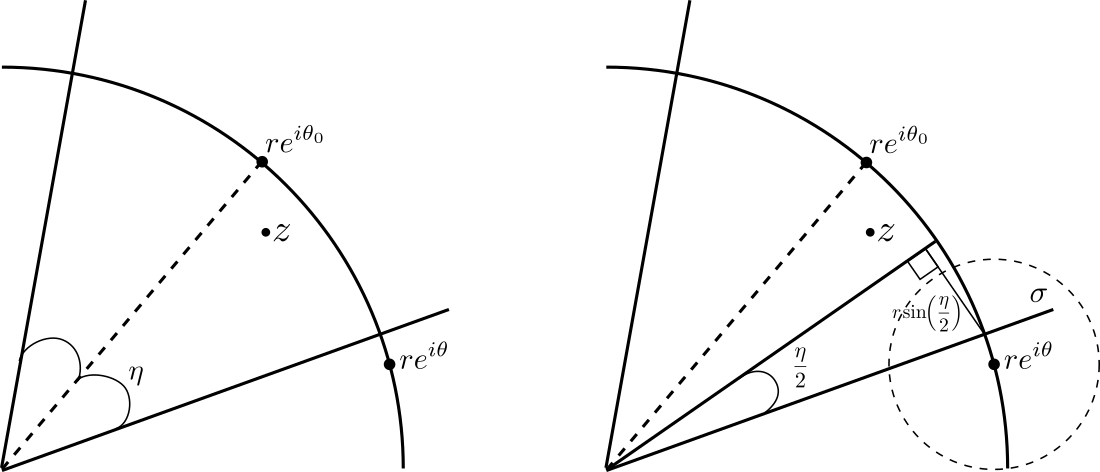
\includegraphics[scale=0.8]{Images/dirichlet_prob_lemma.png}
        \caption{Distance between $z$ and $re^{i\theta}$ is at least $r \sin\left(\frac{\eta}{2}\right)$}
        \label{fig:dirichlet-prob-lemma}
    \end{figure}
\end{proof}

Given this lemma we now consider (using the fact that the integral of the Poisson kernel is 1). 
\begin{align*}
    F(z) - f(\theta_0) &= \frac{1}{2\pi} \int_0^{2\pi} f(\theta) \frac{r^2 - \abs{z}^2}{\abs{re^{i\theta_0} - z}^2} d\theta - \int_0^{2\pi} \frac{1}{2\pi} f(\theta_0) \frac{r^2 - \abs{z}^2}{\abs{re^{i\theta_0} - z}^2} d\theta\\
    &= \frac{1}{2\pi} \int_{\abs{\theta - \theta_0} \leq \eta} (f(\theta) - f(\theta_0)) \frac{r^2 - \abs{z}^2}{\abs{re^{i\theta_0} - z}^2} d\theta + \frac{1}{2\pi} \int_{\abs{\theta - \theta_0} > \eta} (f(\theta) - f(\theta_0)) \frac{r^2 - \abs{z}^2}{\abs{re^{i\theta_0} - z}^2} d\theta
\end{align*}
We can do this split for any $\eta$ so now we need to decide what a good choice of $\eta$ should be. Suppose we are given some $\epsilon > 0$. By continuity of $f$, we know $\sup_{\abs{\theta - \theta_0} \leq \eta} \abs{f(\theta) - f(\theta_0)}$ can be made as small as we like by choosing $\eta$ appropriately. So in particular we can easily choose an $\eta$ so the first integral is less than $\frac{\epsilon}{2}$ (we just integrate over a sufficiently small arc). With this choice of $\eta$ we get 
$$\abs{\frac{1}{2\pi} \int_{\abs{\theta - \theta_0} > \eta} (f(\theta) - f(\theta_0)) \frac{r^2 - \abs{z}^2}{\abs{re^{i\theta_0} - z}^2} d\theta} \leq M \cdot \frac{1}{2\pi}\int_{\abs{\theta - \theta_0} > \eta}\frac{r^2 - \abs{z}^2}{\abs{re^{i\theta_0} - z}^2} d\theta $$
which we can make arbitrary small by the lemma above. In particular we can make it smaller than $\frac{\epsilon}{2}$ which gives us continuity of $F$ on the boundary.
\end{proof}

In fact, we can use this to completely characterise harmonic functions via the mean value property.
\begin{theorem}
    If $f$ is a continuous function on an open set $\Omega$ such that it satisfies the Mean Value Property, then $f$ is harmonic.
\end{theorem}
\begin{proof}
    It suffices to show that $f$ is locally harmonic at every point. Let $z \in \Omega$ be arbitrary and $D$ be a disk centered at $z$ so that $D \subset \Omega$. We know that $f|_{\partial D}$ is continuous and therefore by the above theorem there exists a continuous $F$ which agrees with $f$ on the boundary of $D$ and is harmonic on the interior of $D$. Since $F$ and $f$ satisfy the maximum modulus principle so does $F - f$. But since $F - f$ is 0 on the boundary, it must be identically 0 on $D$, implying that $f = F$ is harmonic.
\end{proof}

\section{Runge's Approximation Theorem}
We end with a powerful statement that uses Cauchy's Integral Formula in a rather interesting way. 

The question we wish to ask is whether a holomorphic function on a compact set can be uniformly approximated using polynomials (we know the analogous statement is true for real numbers by Stone-Weirstrass Theorem). In some cases, this can be done. For example, if we have a power series expansion on the entire compact set, then the partial sum will approximate the function uniformly. On the other hand, we have cases where there is definitely no polynomial approximation. Consider for example the function $f(z) = z^{-1}$ which we might wish to approximate on the unit circle $S^1$. Suppose $p_n(z)$ form a sequence of polynomials that uniformly converge to $f$. But we see that the integral over $S^1$ of $f$ is $2\pi i$ while the integral over $S^1$ of $p_n(z)$ is $0$ for all $n$. Thus $p_n$ could not have converged to $f$. We will see that this is more or less the only thing that can go wrong. In other words, we can always approximate holomorphic functions by polynomials or by rational functions with poles outside the compact set.

Before stating and proving the theorem, let us first prove the following lemma.
\begin{lemma}\label{lem:poly-approx-along-curve}
        If $\C \setminus K$ is connected and $z_0 \notin K$ then $\frac{1}{z - z_0}$ can be approximated on $K$ by polynomials.
    \end{lemma}
    \begin{proof}
        Let $D$ be a disk centered at 0 containing $K$. The first case is when $z_0$ is not in $D$. Then
        $$\frac{1}{z - z_0} = -\frac{1}{z_0} \cdot \frac{1}{1 - \frac{z}{z_0}} = - \sum_{n = 0}^\infty \frac{z^n}{z_0^{n + 1}}$$
        So the partial sum of the series above form the desired polynomials (we need $z_0$ outside $D$ to ensure that $\abs{\frac{z}{z_0}} < 1$).

        For the second case, suppose $z_0$ is in $D$. By the first case, it suffices to show that $\frac{1}{z - z_0}$ can be uniformly approximated on $K$ by polynomials in $\frac{1}{z - z_1}$ where $z_1$ is some point outside $D$. Since $\frac{1}{z - z_1}$ itself can be approximated by polynomials this allows us to do the same for $\frac{1}{z - z_0}$. 

        \begin{figure}
            \centering
            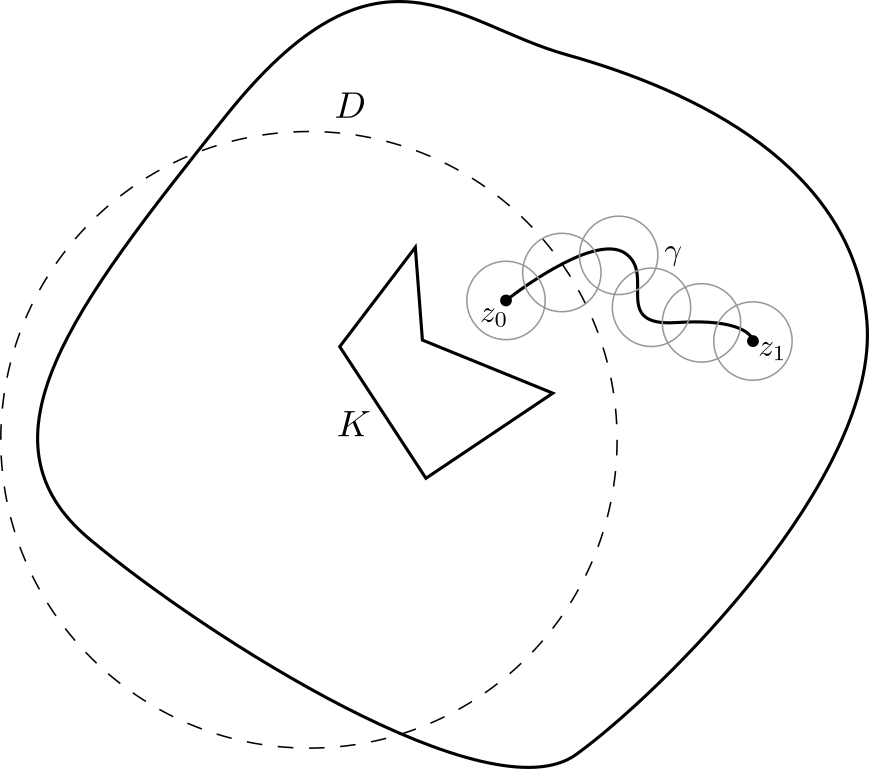
\includegraphics[scale=0.6]{Images/poly_approx_along_curve.png}
            \caption{Successively approximate by polynomials in $\frac{1}{z - w}$ along the curve}
            \label{fig:poly-approx-along-curve}
        \end{figure}
        
        Let $\gamma$ be a path joining $z_0$ and $z_1$ (such a path exists by connectedness of $\C \setminus K$). Choose a sequence of points $\{w_1, \dots, w_k\}$ on the curve such that $\abs{w_{i + 1} - w_i} < \frac{1}{2} d(\gamma, K) =: \delta$. Finally we reduce the problem even further to showing that if $w \in \gamma$ and $\abs{w - w'} < \delta$ then $\frac{1}{z - w}$ can be approximated uniformly in $K$ by polynomials in $\frac{1}{z - w'}$. This is easy to see by our usual geometric series argument since
        \begin{align*}
            \frac{1}{z - w} = \frac{1}{z - w' + w' - w} = \frac{1}{z - w'} \cdot \frac{1}{1 - \frac{w - w'}{z - w'}} = \sum_{n = 0}^\infty \frac{(w - w')^n}{(z - w')^{n + 1}}
        \end{align*}
    \end{proof}

\begin{theorem}[Runge's Approximation Theorem]
    Let $\Omega \subset \C$ be open and let $K$ be a compact subset of $\Omega$. Let $f$ be a holomorphic function on $\Omega$. Then
    \begin{enumerate}
        \item $f$ can be approximated on $K$ uniformly by rational functions with poles in $\C \setminus K$
        \item If $\C \setminus K$ is connected, then $f$ can be uniformly approximated on $K$ by polynomials instead
    \end{enumerate}
\end{theorem}
\begin{proof}
    First, we choose a grid of squares of side length less than $d(K, \C \setminus \Omega)$ so that any square intersecting $K$ lies inside $\Omega$. Let $\mathcal{Q} := \{Q_1, \dots, Q_M\}$ be squares that intersect $K$ (all with positively oriented boundaries). Let $\gamma_1, \dots, \gamma_n$ be boundary segments of $Q_j$ that don't belong to two adjacent squares in $\mathcal{Q}$. Then each $\gamma_l$ is contained in $\Omega$ (because of how we chose the grid) and does not intersect $K$ (if it did there would be 2 adjacent squares containing $\gamma_l$).

    \begin{figure}[ht]
        \centering
        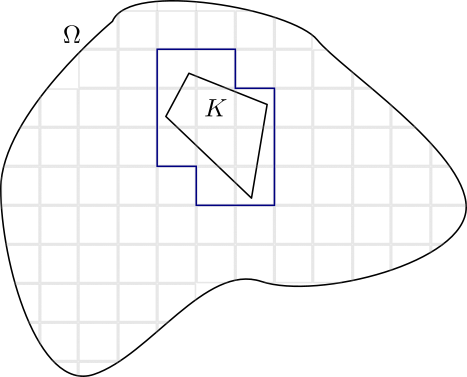
\includegraphics[scale=0.9]{Images/runge_approx_grid.png}
        \caption{Draw a fine grid so that squares intersecting $K$ are entirely inside $\Omega$. The blue line indicates boundary elements of $Q_j$ that do not belong to two adjacent squares}
        \label{fig:runge-approx-grid}
    \end{figure}

    Then we claim that 
    $$f(z) = \frac{1}{2\pi i} \sum_{l = 1}^n \int_{\gamma_l} \frac{f(\zeta)}{\zeta - z} d\zeta$$
    In order to verify this, first suppose $z$ is an element of $Q_1 \cup \dots \cup Q_M$ such that it does not lie on the boundary of any $Q_j$. Then if $z \in Q_j$ we see by Cauchy's Integral Formula that
    $$ \frac{1}{2\pi i} \int_{\partial Q_m} \frac{f(\zeta)}{\zeta - z}d\zeta = 
    \begin{cases}
    f(z) &\text{ if } m = j\\
    0 &\text{otherwise}
    \end{cases}$$
    This means that 
    $$f(z) = \frac{1}{2\pi i} \sum_{m = 1}^M \int_{Q_m} \frac{f(\zeta)}{\zeta - z}d\zeta = \frac{1}{2\pi i} \sum_{n = 1}^N \int_{\gamma_n} \frac{f(\zeta)}{\zeta - z}d\zeta$$
    where the last inequality follows from the fact that if a boundary is shared by two of the $Q_j$ then the integral over it cancels out. The statement holds for $z$ even if they lie on the boundary of some $Q_j$ by continuity.

    Then we can consider each term in the sum separately reducing the problem to the lemma below which more or less immediately tells us when polynomial approximations can be found.
    \begin{lemma}
        Suppose $\gamma$ is a line segment in $\Omega \setminus K$. Then
        $$\int_{\gamma} \frac{f(\zeta)}{\zeta - z} d\zeta$$
        can be uniformly approximated on $K$ by rational functions with poles on $\gamma$.
    \end{lemma}
    \begin{proof}
        We see that
        $$\int_\gamma \frac{f(\zeta)}{\zeta - z}d\zeta = \int_0^1 \frac{f(\gamma(t))}{\gamma(t) - z}\gamma'(t) dt$$
    The integrand $F(z, t)$ is a continuous function on a compact set $K \times [0, 1]$ and is therefore uniformly continuous. Therefore for any $\epsilon > 0$ we can find some $\delta$ such that whenever $\abs{t_1 - t_2} < \delta$, we have
    $$\sup_{z \in K} \abs{F(z, t_1) - F(z, t_2)} < \epsilon$$
    This exactly means that the Riemann sums of $\int_0^1 F(z, t) dt$ converge to the integral uniformly on $K$. But each term in the Riemann sum is of the form
    $$ \frac{f(\gamma(t_i))}{\gamma(t_i) - z}\gamma'(t_i) \cdot (t_{i + 1} - t_i) $$
    which is a rational function (in fact a very simple one since it is of the form $\frac{A}{B + z}$) with a pole $\gamma(t_i)$. This is true for each term of the sum and since the sum of rational functions is rational we conclude that the Riemann sums are rational functions with poles on $\gamma$ that uniformly approximate the holomorphic function $f$.
    \end{proof}

    The previous lemma, \autoref{lem:poly-approx-along-curve}, tells us that under nice conditions (namely $\C \setminus K$ being connected) rational functions of the form $\frac{1}{z - z_0}$ can be approximated by polynomials. Above we have shown that any holomorphic function can be approximated by polynomials in $\frac{1}{z - z_0}$. Thus if $\C \setminus K$ is connected we can approximate $f$ using polynomials.
\end{proof}